%%%% fatec-article.tex, 2024/03/10

\documentclass[
  a4paper,%% Tamanho de papel: a4paper, letterpaper (^), etc.
  12pt,%% Tamanho de fonte: 10pt (^), 11pt, 12pt, etc.
  english,%% Idioma secundário (penúltimo) (>)
  brazilian,%% Idioma primário (último) (>)
]{article}

%% Pacotes utilizados
\usepackage[]{fatec-article}
\usepackage{float}

%% Início do documento
\begin{document}
\vspace{8cm}
\begin{center}
    \large \textbf{\title{ARTEFATOS DO PROJETO DE SOFTWARE}}
\end{center}

\maketitle

\break

\tableofcontents

\break


%exemplo da forma de organização das seções e subseções, você deverá adaptar o template para a realidade do seu projeto.

\section*{Diagramas UML}
    Nesta seção serão apresentados os diagramas da UML utilizados para a modelagem do sistema desenvolvido. Dentre os diagramas utilizados, pode-se citar: Diagrama de Caso de Uso, Diagrama de Classe e Diagrama de Objetos.
    
    \subsection*{Diagrama de Caso de Uso}
    \addcontentsline{toc}{section}{Diagrama de Caso de Uso}

    Este diagrama de caso de uso representa a interação entre os principais atores: Usuário, APi e IA Preditiva. Além dos casos de uso associados ao sistema.
    O fluxo inicia com o Usuário, que aciona o caso de uso “Inicia o teste”. A partir dessa ação, o sistema executa uma sequência de processos automatizados que incluem o “Rastreamento ocular durante as fases” e a “Coleta das métricas”. Em seguida, os dados obtidos são enviados ao banco de dados pela API.
    Após o armazenamento, a IA Preditiva coleta os resultados e realiza a análise dos dados. Com base nessa análise, o sistema gera um resultado interpretativo sobre o desempenho atencional do participante.  Por fim, o caso de uso “Exibe o resultado para o usuário” completa o ciclo, apresentando o relatório obtido no teste.



\begin{figure}[H]
\centering
\caption{Diagrama de caso de uso}%
\label{fig:caso-de-uso}
 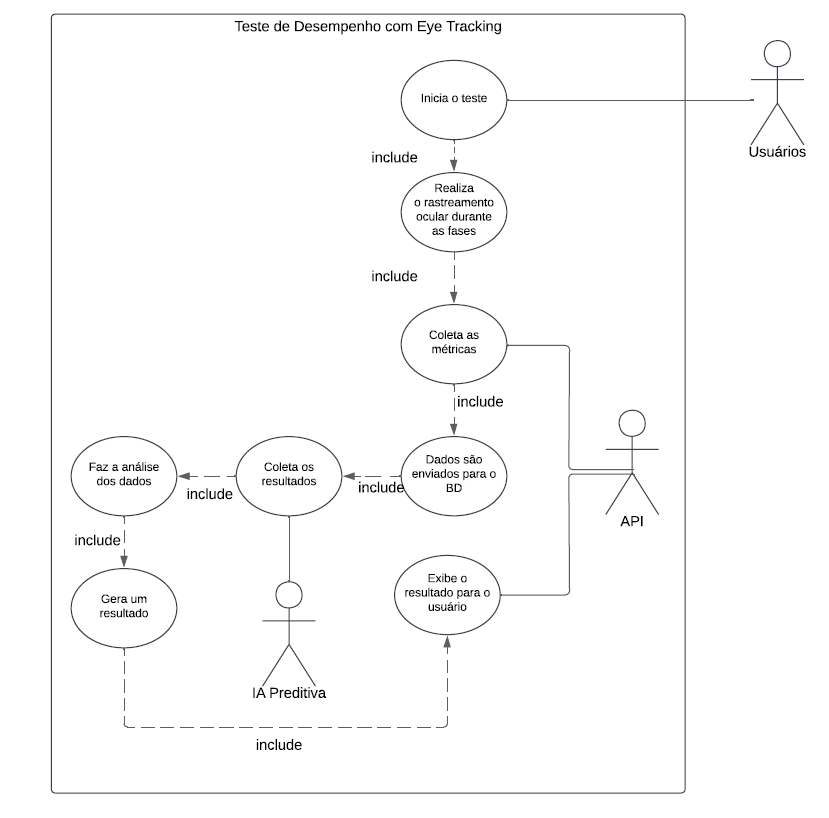
\includegraphics[width=1.1\textwidth]{Logos/caso-de-uso.png}
\SourceOrNote{Do próprio autor (2025)}
\end{figure}


    Esse diagrama sintetiza o comportamento funcional do sistema, evidenciando a integração entre os módulos de captura de dados via eye tracking, processamento por inteligência artificial e comunicação por meio de API. O artefato é fundamental para compreender a estrutura lógica e o fluxo de informações dentro da aplicação proposta.
    
    \subsection*{Diagrama de Classe}
    \addcontentsline{toc}{section}{Diagrama de Classe}

    Este Diagrama de Classe modela a estrutura de dados e as principais entidades do sistema de rastreamento ocular para avaliação de atenção.
    O diagrama ilustra quatro classes principais: Usuário, que armazena dados básicos de identificação, como nome, idade e sexo, além disso, contém os métodos logar(), logout(), jogar() e visualizarPréDiagnóstico(). A classe denominada Fases, que define as carcterísticas de cada fase do jogo, incluindo atributos como nome da fase (podendo variar entre "Fase 1", "Fase 2" e "Fase 3"), descrição, tempoTotal e o tipoAtençãoAvaliada. O método para esta classe é o iniciar() para começar uma fase do jogo. Possui a classe de Inteligência Aritifical (IA), que armazena os resultados brutos do rastreamento ocular, como dataTeste, usuário, métricas de foco (TempoInícioFoco, tempoMínimoFoco, tempoTotal, acertos), e contagens de erros (errosPorOmissão, errosPorComissão) todos como inteiros. A IA é responsável pelo processamento dos resultados e diagnóstico através dos métodos analisarResultados() e gerarPréDiagnóstico(). Por fim, a classe PréDiagnóstico que guarda o resultado final da avaliação de atenção para um usuário em uma determinada fase, incluindo usuário, fase, comentário e um valor de precisão. O pré diagnóstico é exibido ao usuário através do método mostrarPréDiagnósticoUsuário().

    \begin{figure}[H]
\centering
\caption{Diagrama de classe}%
\label{fig:diagrama-de-classe}
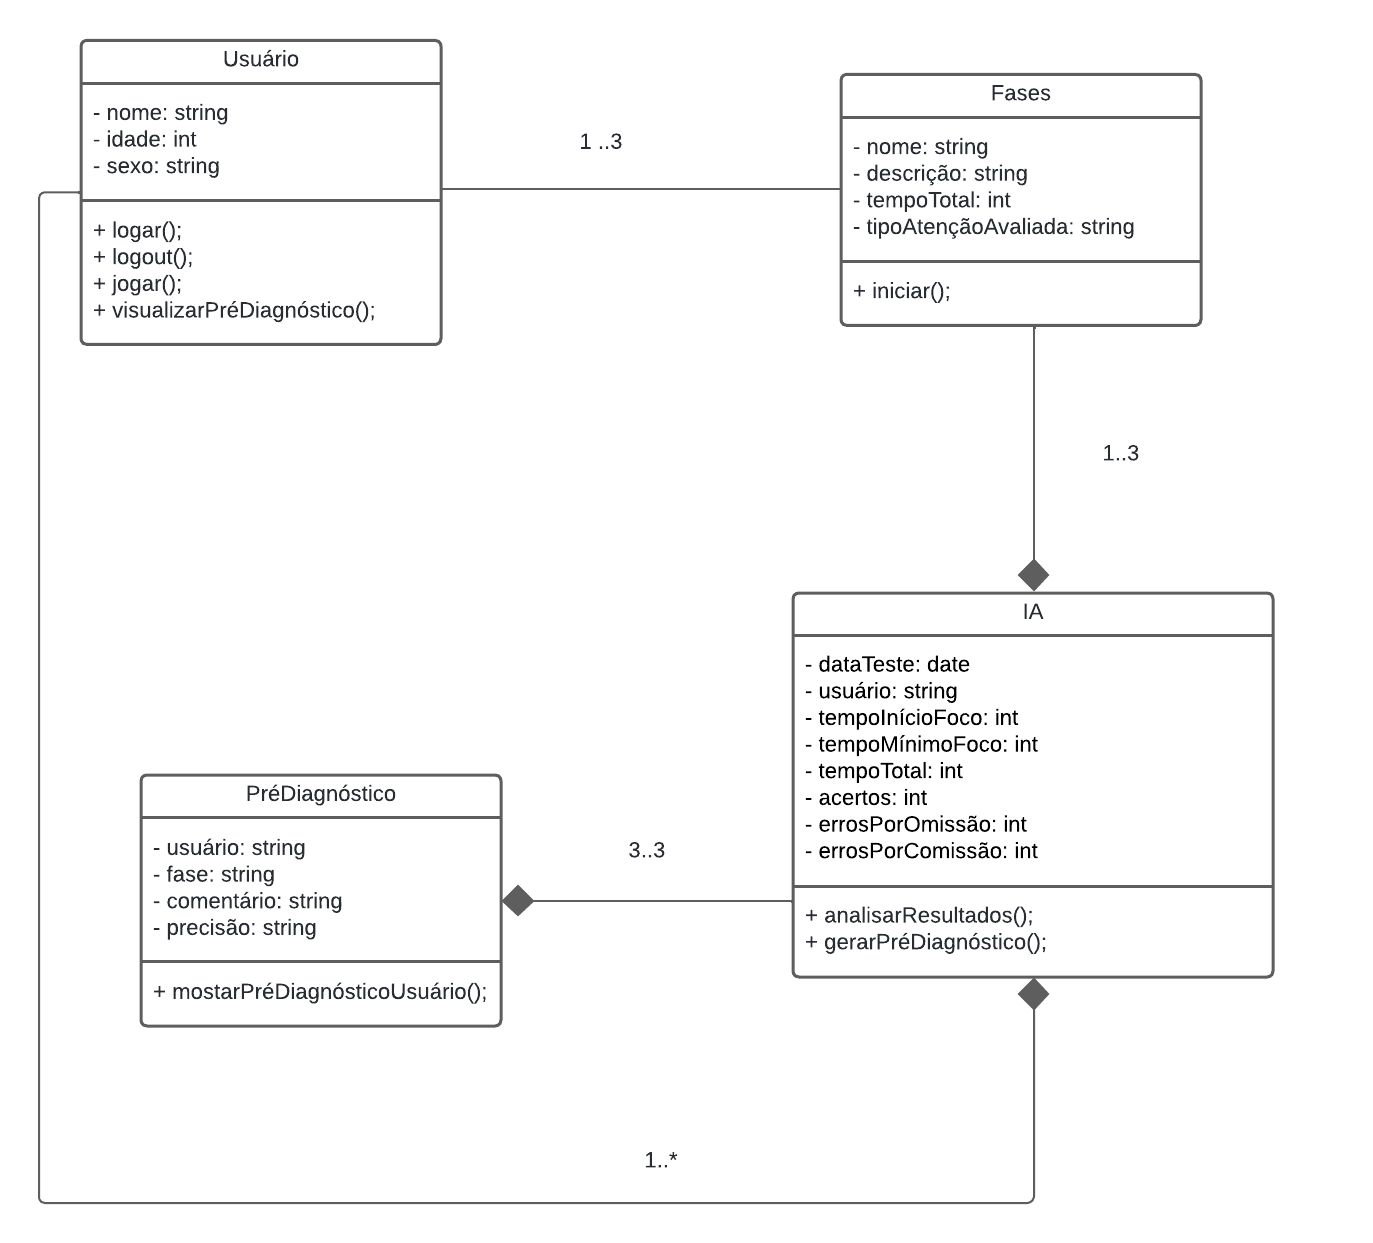
\includegraphics[width=0.8\textwidth]{Logos/diagrama-de-classe.png}
\SourceOrNote{Do próprio autor (2025)}
\end{figure}

    O diagrama de classe estabelece as seguintes associações e composições entre as classes: O relacionamente entre Usuário e Fases possui uma cardinalidade de uma para três, indicando que um usuário pode participar de até três fases do jogo. De forma semelhante, a associação entre Fases e IA também é de uma para três, refletindo que cada fase gera um conjunto de dados de rastreamento ocular. A classe IA está associada à classe PréDiagnóstico em uma relação de três para três, indicando que cada conjunto a IA pode gerar no mínimo e no máximo três pré diagnósticos, pois é um para cada fase do jogo. Por fim, a composição entre Usuário e PréDiagnóstico é de um para muitos, indicando que um usuário pode ter múltiplos pré diagnósticos ao longo do tempo.

    \subsection*{Diagrama de Objetos}
    \addcontentsline{toc}{section}{Diagrama de Objetos}

    O Diagrama de Objetos representa uma instância específica do sistema em execução, ilustrando os objetos concretos e seus relacionamentos em um determinado momento. Este diagrama exemplifica um cenário real do jogo, onde um usuário específico, identificado como "Manuela Santos", de 10 anos e sexo feminino, interage com uma das fases do sistema de avaliação de atenção.
    
    A instância do usuário está associada a um objeto de fase específico, denominada Fase 1, onde deve-se manter o olhar em cinco estrelas por 5s em cada com o tempo total de 60s e, que avalia a "Atenção Sustentada".
    
    Para esta fase executada, o sistema gera uma instância da classe IA contendo as métricas coletadas durante o rastreamento ocular, armazenando dados como tempo de início de foco, tempo mínimo de foco, tempo total, quantidade de acertos, erros por omissão e erros por comissão. Com base nesses dados, o sistema gera uma instância de pré-diagnóstico, associada à fase executada e contendo o comentário avaliativo "Atenção dentro do esperado", juntamente com o valor de precisão do olhar capturado.
    
    \begin{figure}[H]
\centering
\caption{Diagrama de objetos}%
\label{fig:diagrama-de-objetos}
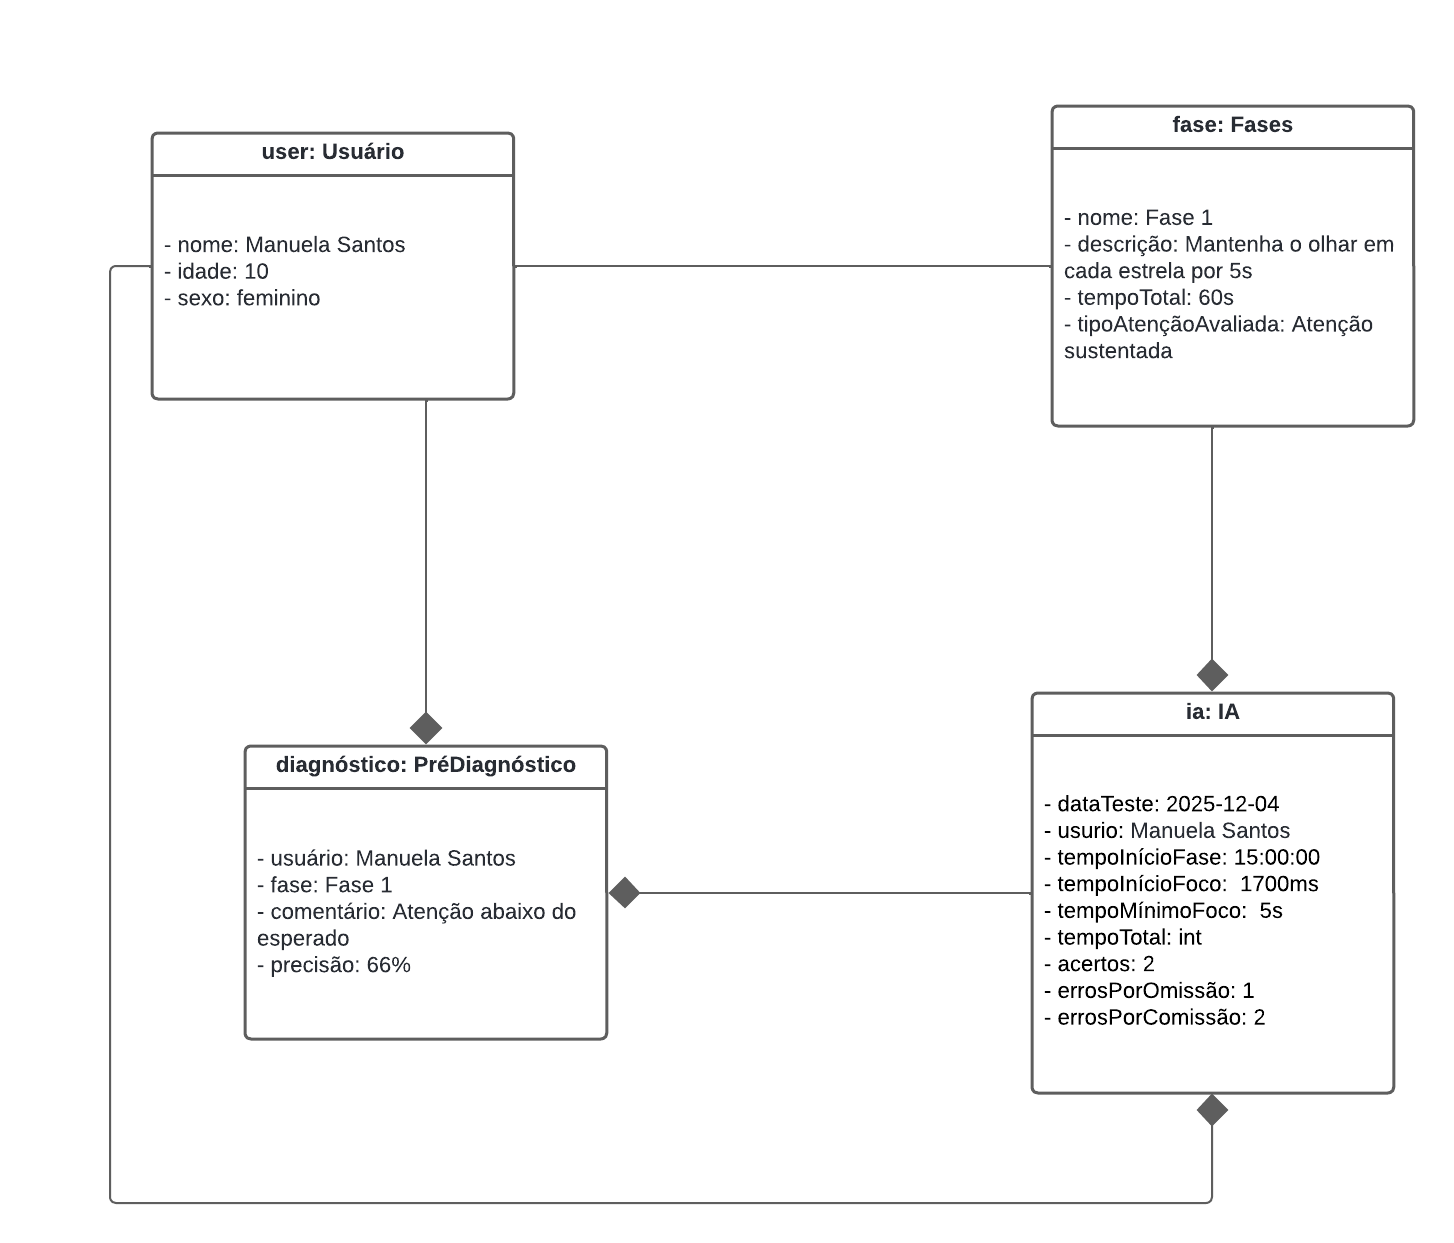
\includegraphics[width=0.8\textwidth]{Logos/diagrama-de-objetos.png}
\SourceOrNote{Do próprio autor (2025)}
\end{figure}

    Este diagrama ilustra concretamente como os dados fluem desde a interação do usuário com uma fase do jogo até a geração do pré-diagnóstico individualizado, demonstrando a aplicação prática da estrutura modelada no Diagrama de Classes através de uma instância específica do sistema.

    \subsection*{Diagrama de banco de dados}
    \addcontentsline{toc}{section}{Diagrama de banco de dados}

    O modelo conceitual representa a estrutura de armazenamento de dados para o sistema de rastreamento ocular e análise de atenção.Esta arquitetura foi projetada acomoda os dados complexos gerados durante as três fases de testes do sistema.

    O banco de dados é composto por seis coleções principais inter-relacionadas:

    \begin{figure}[H]
\centering
\caption{Diagrama de banco de dados}%
\label{fig:diagrama-de-banco-de-dados}
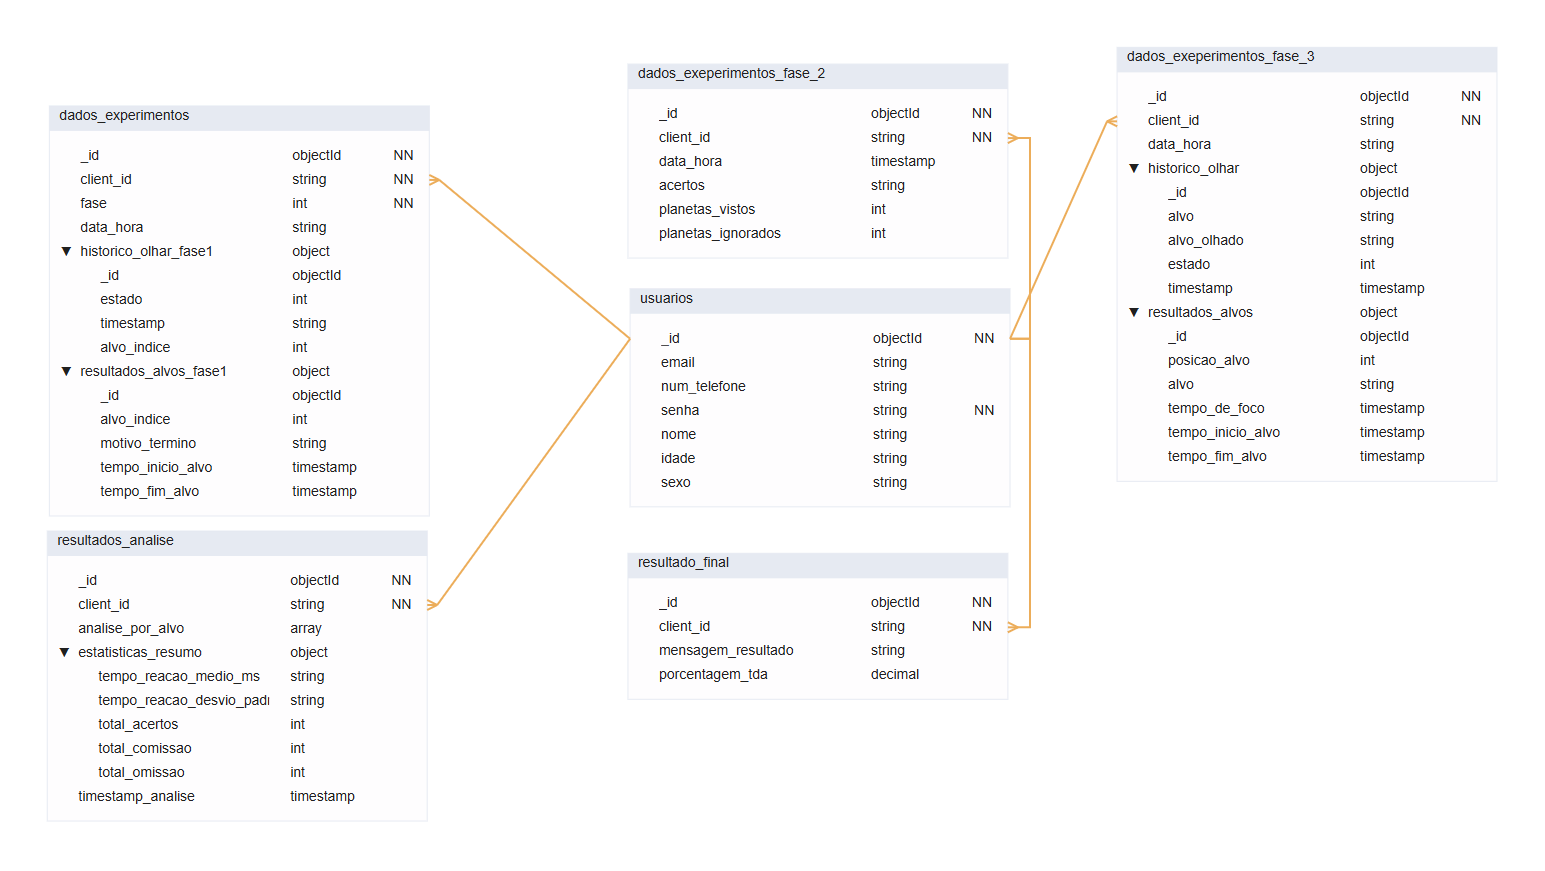
\includegraphics[width=0.8\textwidth]{Logos/mongo.png}
\SourceOrNote{Do próprio autor (2025)}
\end{figure}

    


\begin{itemize}
    \item \textbf{usuarios}: Armazena informações de cadastro das crianças que jogarão as fases. Os campos incluem: \texttt{\_id}, \texttt{email}, \texttt{num\_telefone}, \texttt{senha}, \texttt{nome}, \texttt{idade}, e \texttt{sexo}.

    \item \textbf{dados\_experimentos} (Fase 1): Registra dados brutos dos experimentos realizados na primeira fase. Contém dois subdocumentos principais: \texttt{historico\_olhar\_fase1} (para a sequência temporal do olhar) e \texttt{resultados\_alvos\_fase1} (para resultados específicos por alvo).

    \item \textbf{dados\_experimentos\_fase\_2} (Fase 2): Coleção dedicada aos dados da segunda fase, focando em métricas de desempenho. Os campos principais são: \texttt{acertos}, \texttt{planetas\_vistos}, e \texttt{planetas\_ignorados}.

    \item \textbf{dados\_experimentos\_fase\_3} (Fase 3): Coleção para dados da terceira fase. Contém dois subdocumentos principais: \texttt{historico\_olhar} (para a trajetória completa do olhar) e \texttt{resultados\_alvos} (para métricas temporais por alvo específico).

    \item \textbf{resultados\_analise}: Contém resultados processados e análises estatísticas da primeira fase. Inclui o array \texttt{analise\_por\_alvo} para análise granular e um subdocumento \texttt{estatisticas\_resumo} com métricas consolidadas (tempos de reação, totais de acertos, comissão e omissão).

    \item \textbf{resultado\_final}: Apresenta o diagnóstico consolidado final, baseado nos dados de todas as três fases. Inclui uma \texttt{mensagem\_resultado} descritiva e a \texttt{porcentagem\_tda} quantitativa.
\end{itemize}


O modelo segue um fluxo lógico de processamento de dados definido:
\begin{enumerate}
    \item Coleta de Dados do Usuário.
    \item Coleta de Dados Experimentais (Fases 1, 2 e 3).
    \item Análise Estatística.
    \item Geração do Resultado Final e Diagnóstico (preenchido por análise de IA).
\end{enumerate}

 Esta estrutura permite uma análise compreensiva do desempenho de atenção através do rastreamento ocular, desde a coleta bruta de dados até a geração de diagnósticos individuais, mantendo a flexibilidade necessária para acomodar os diferentes tipos de dados gerados em cada fase experimental.

\section*{Canvas}
    \addcontentsline{toc}{section}{Canvas}
    
    Esse modelo de negócios foi estruturado de acordo com os nove blocos do Canvas, permitindo visualizar de forma integrada os principais elementos que compõem a proposta de valor, os recursos, os canais e a estrutura operacional do projeto.

    A Proposta de Valor consiste em oferecer um jogo sério que, de maneira gamificada, avalia o desempenho atencional e fornece feedbacks personalizados aos usuários, auxiliando em processos de triagem e apoio diagnóstico.

    Os Canais de entrega envolvem o uso de computadores com câmeras integradas e acesso à internet, com o sistema hospedado em servidor remoto. O Relacionamento com o Cliente baseia-se em experiências interativas e intuitivas, com geração de pré-diagnósticos rápidos e relatórios claros.

    As Fontes de Renda incluem a comercialização do software como serviço (modelo de assinatura mensal), oferecendo relatórios automatizados, alto nível de interatividade e conveniência para profissionais da área.

    Entre os Recursos-Chave, destacam-se a infraestrutura digital (website e hospedagem), a divulgação por meio de anúncios na internet e o compartilhamento de recomendações entre usuários.

    As Atividades-Chave compreendem o desenvolvimento e manutenção do sistema, a aplicação dos testes em ambientes clínicos e educacionais, e a interação direta com o usuário final.

    Os Parceiros-Chave incluem provedores de hospedagem, fornecedores de infraestrutura digital e plataformas de divulgação online.

    Por fim, a Estrutura de Custos abrange despesas fixas com hospedagem, infraestrutura e publicidade, sustentadas pelo modelo de assinatura mensal para acesso ao serviço.

\begin{figure}[H]
\centering
\caption{Canvas}%
\label{fig:canvas}
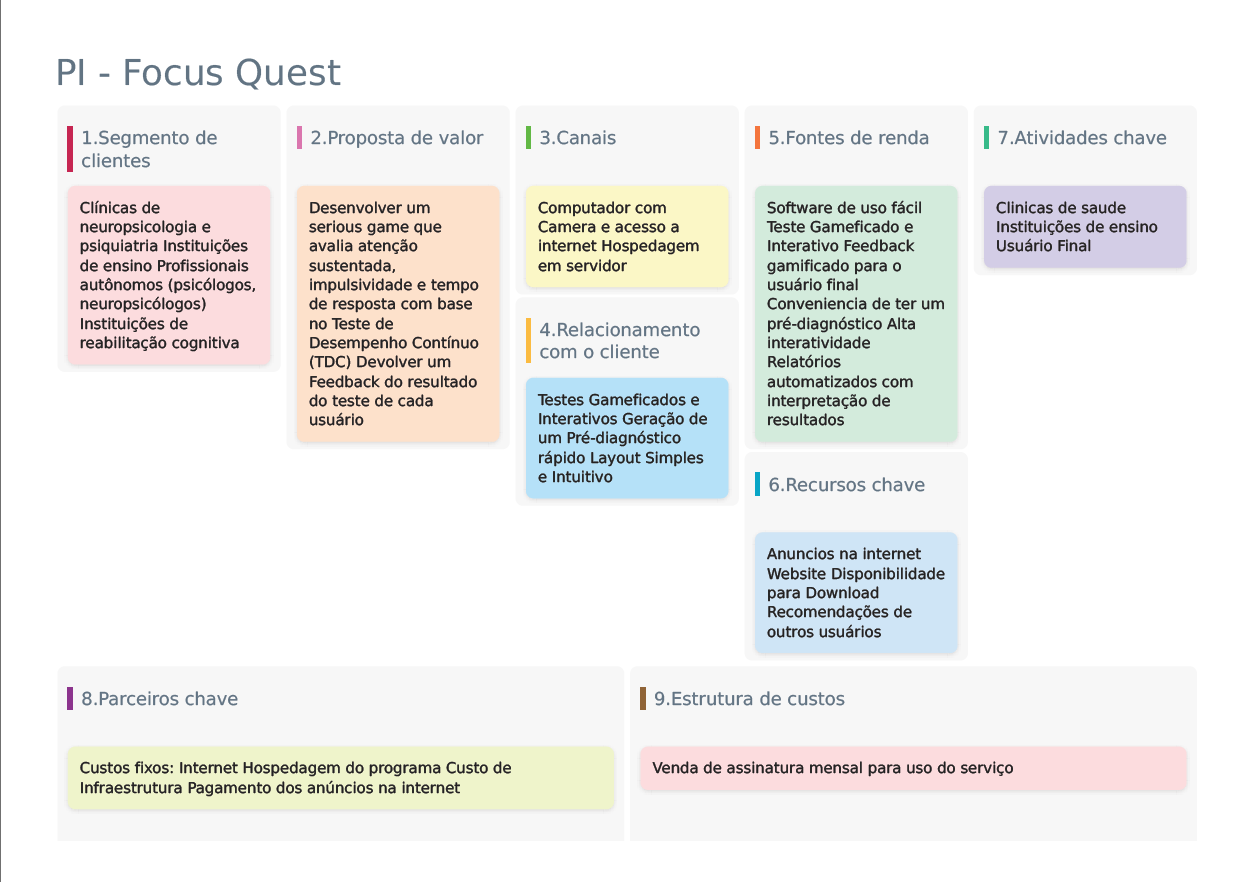
\includegraphics[width=1.1\textwidth]{Logos/canvas.png}
\SourceOrNote{Do próprio autor (2025)}
\end{figure}

    Esse artefato auxilia na visualização estratégica do projeto Focus Quest, evidenciando sua viabilidade técnica e comercial, além de integrar as dimensões tecnológicas, clínicas e de mercado do produto proposto.

\section*{Diagrama de redes}
    \addcontentsline{toc}{section}{Diagrama de Redes}
    
    Este diagrama representa a estrutura de redes completa do sistema, desde o funcionamento local no computador do usuário até a coleta e o processamento dos dados do lado do servidor.

    O processo inicia-se no PC do Usuário, onde é executado o \textit{software} do teste gamificado e ocorre a captura dos dados visuais por meio do módulo de \textit{Eye Tracking}, responsável por registrar o movimento ocular do participante durante as tarefas do TDC. Esses dados são enviados para a rede local e encaminhados a um Roteador/\textit{Switch}, que gerencia o tráfego e redireciona as informações para a camada de comunicação externa.

    A seguir, o ISP (\textit{Internet Service Provider}, em português, Provedor de Servico de Internet) encaminha os dados até o ambiente em nuvem, onde está hospedada a \textit{API}, responsável pela coleta e organização das métricas capturadas. As informações processadas são então armazenadas em um banco de dados \textit{NoSQL}.

    Na sequência, os dados são processados pela camada de Inteligência Artificial de Aprendizado Profundo (\textit{Deep Learning AI}), que realiza análises preditivas e interpretações automatizadas dos resultados. Após o processamento, as informações podem ser retornadas ao sistema do usuário ou disponibilizadas para visualização em relatórios analíticos

\begin{figure}[H]
\centering
\caption{Diagrama de redes}%
\label{fig:diagrama-de-redes}
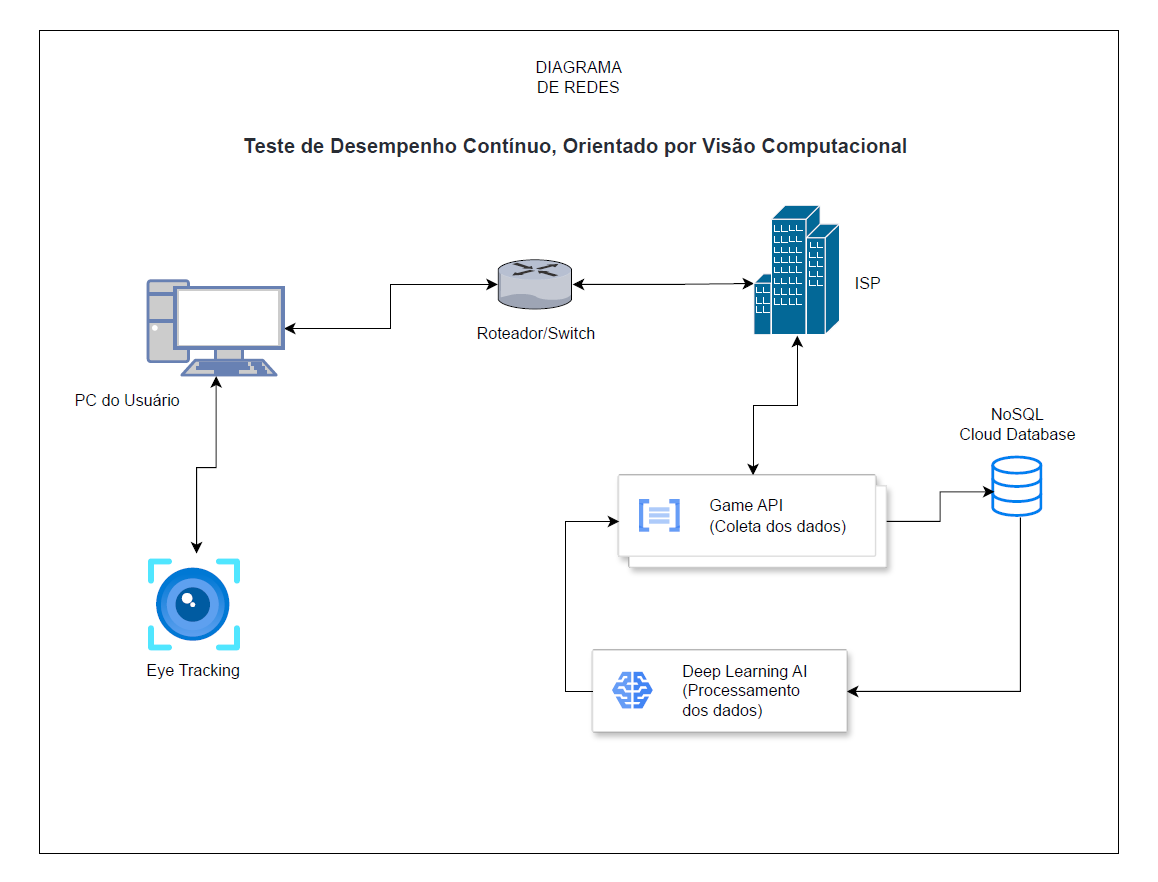
\includegraphics[width=1.1\textwidth]{Logos/diagrama-de-redes.png}
\SourceOrNote{Do próprio autor (2025)}
\end{figure}

    Esse diagrama representa a infraestrutura lógica do sistema, evidenciando a integração entre os módulos de coleta via \textit{eye tracking}, comunicação em nuvem, análise de dados com IA e armazenamento distribuído.

\section*{Análise SWOT}
    \addcontentsline{toc}{section}{Análise SWOT}

Nos pontos fortes, destaca-se o domínio da equipe sobre as tecnologias empregadas, o que garante eficiência no desenvolvimento e confiabilidade nos resultados. O sistema apresenta valor prático ao auxiliar no pré-diagnóstico do Déficit de Atenção, além da integração com o rastreamento ocular, que amplia a precisão da análise comportamental. Esses fatores reforçam a relevância científica e tecnológica da solução.

Nos pontos fracos, observa-se que a principal limitação está na dependência de condições técnicas externas, como a qualidade da câmera e a iluminação do ambiente, que podem comprometer o desempenho do rastreamento ocular. Além disso, a obtenção de uma base de dados confiável é um processo rigoroso, exigindo tempo e validação ética, o que pode retardar a evolução do sistema.

As oportunidades demonstram um cenário favorável de aplicação prática e divulgação. Clínicas e instituições de saúde podem adotar o sistema como ferramenta de apoio diagnóstico, enquanto a originalidade da abordagem aumenta seu potencial de destaque em feiras de tecnologia e ambientes acadêmicos. Isso cria espaço para futuras parcerias e aprimoramentos.

\begin{figure}[H]
\centering
\caption{Análise SWOT}%
\label{fig:analise-swot}
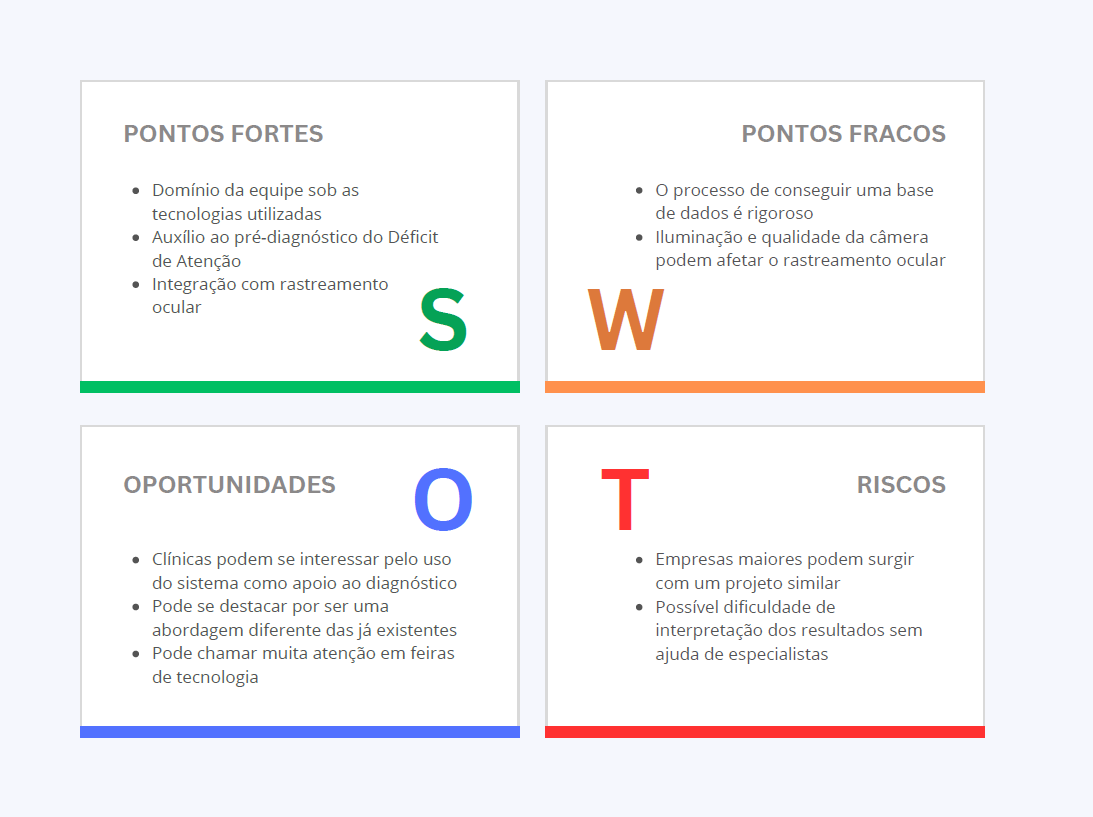
\includegraphics[width=1.1\textwidth]{Logos/swot.png}
\SourceOrNote{Do próprio autor (2025)}
\end{figure}

    Por fim, os riscos estão ligados à competitividade do mercado e à necessidade de interpretação especializada dos resultados. Projetos semelhantes podem surgir em empresas com maior capacidade de investimento, e a dependência de especialistas pode limitar o uso autônomo do sistema.

\end{document}

